\subsubsection{Shopping List Browser}
The Shopping List Browser is found in the third tab in our HomeActivity. It was
implemented in the following manner:
\begin{description}
\item[Shopping List Creator] This was implemented as ShopFragment and allows the
users to add products with a editable quantity to a shopping list. It also
contains a search button which will search for stores stocking the products and
calculate the cost of the products at them before presenting the information in
StoreFragment. 
\item[Store Viewer] This was implemented as StoreFragment which displays a
list of stores which were found along with the total cost of the products at
that store. Each store in the list is clickable and takes the user to
BrowseFragment, displaying that store's shopping list products. There is also a
map button which takes the user to the MapsActivity after the user has chosen
the store which they need directions for.
\end{description}
\begin{figure}[h!]
\centering
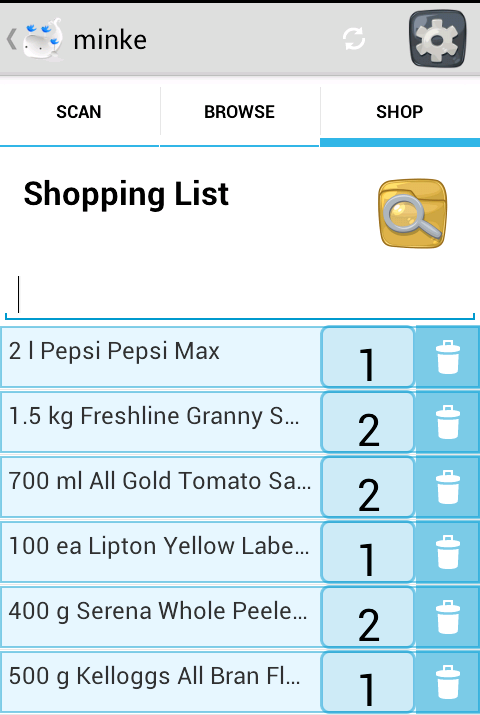
\includegraphics[width=0.3\textwidth]{shop-list.png}
\caption{Shopping list creation.}
\end{figure}
